\chapter{Midas: Capacitive Sensing of Custom 2D Layouts}

\begin{quote}
So Midas, king of Lydia, swelled at first with pride when he found he could transform everything he touched to gold...

--- Claudian, \emph{In Rufinem}
\end{quote}

\section{Preamble}

We begin our exploration of the interlink between sensing and geometry at the simple end of our spectra: Midas links 2D geometry, fabricated from conductive material, to capacitance sensing. This chapter focuses on interfaces created on the surface of flat, ruled, and developable 3D objects, where interaction is triggered by a user's direct touch.

An increasing number of consumer products include user interfaces that rely on touch input. We describe Midas, a software and hardware toolkit to support the design, fabrication, and programming of flexible capacitive touch sensors for interactive objects. With Midas, designers first define the desired shape, layout, and type of touch sensitive areas, as well as routing obstacles, in a sensor editor. From this high-level specification, Midas automatically generates layout files with appropriate sensor pads and routed connections. These files are then used to fabricate sensors using digital fabrication processes, e.g., vinyl cutters and conductive ink printers. Using step-by-step assembly instructions generated by Midas, designers connect these sensors to the Midas microcontroller, which detects touch events. No training or initialization are necessary, as Midas performed the initial routing. Once the prototype is assembled, designers can define interactivity for their sensors: Midas supports both record-and-replay actions for controlling existing local applications and WebSocket-based event output for controlling novel or remote applications.  We demonstrate how Midas can be used to create a number of touch-sensitive interfaces.

\begin{figure}
\centering
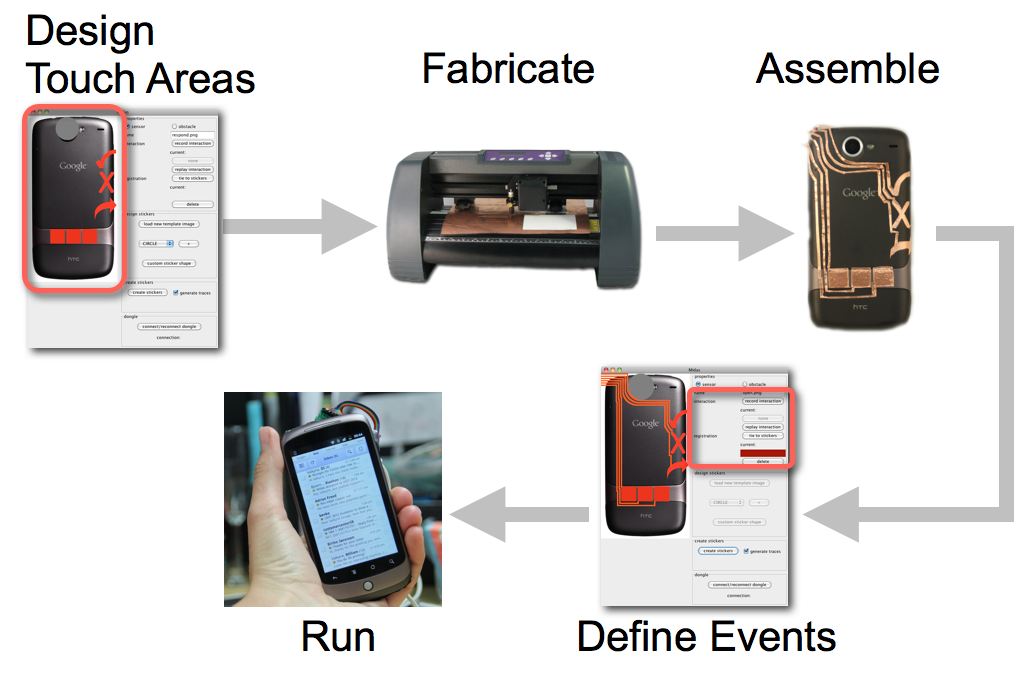
\includegraphics[width=\textwidth]{figures/midas/overview.png}
\caption{Midas enables users to define discrete and continuous touch sensors with custom shapes and layout. It generates fabrication files and assembly instructions. Designers can also define the interaction events of their prototype.}
\label{fig:midas-overview}
\end{figure}

\section{Introduction}

%\valkyrie{How is Midas related to other projects in thesis? How are capacitive interfaces important, how are they seen today}

Ubiquitous, cheap microprocessors have led to a vast increase in consumer products with built-in digital user interfaces. Many of these devices---thermostats, game controllers, and personal medical devices, to name a few---rely on touch sensing to provide input to their user interfaces.

While the rise of the iPhone and subsequent touchscreen-based smartphones has been the most visible use of touch input, these devices rely on software to prototype and create interactions. An app designer can create an interactive graphical user interface using on-screen prototyping tools, purely software with no hardware required. For devices where touch input is not co-located with screen output, for example when a designer wants inputs on the back of a screen (for example to avoid the fat finger problem \cite{baudisch-nanotouch}) or on a device with no screen at all, prototyping becomes much more complicated.

Digital fabrication processes like 3D printing and CNC machining make it easier to prototype the \emph{form} of such products, enabling designers to go directly from a digital 3D model to a physical object. In addition, user interface prototyping tools have lowered the threshold to connect sensors to graphical user interfaces. However, one main limitation of current toolkits such as Phidgets~\cite{greenberg-phidgets}, d.tools~\cite{hartmann-dtools}, .NET Gadgeteer~\cite{villar-gadgeteer}, or Arduino~\cite{arduino} is their reliance on pre-packaged, off-the-shelf sensors such as momentary switches or slide potentiometers. Using pre-packaged sensors has important drawbacks. It {\em constrains exploration}: pre-defined physical form factors restrict the space of realizable designs. For example, available buttons can be too bulky or too small, or sliders may be too long or too short. Most sensors also lack {\em physical flexibility}: they are not easily applied to non-planar surfaces or added to existing objects. Finally, a large {\em gulf of execution} remains between digital design files and physical prototypes: sensors must be manually placed and wired one-by-one. This process is tedious and error-prone; physical prototypes can easily deviate from digital design files if a wire is incorrectly placed or forgotten. While recent research has introduced tools to create touch sensors of different shapes~\cite{holman-tactiletape,hudson-boxes,wimmer-tdr}, their efforts focus on rapidly-constructable, low-fidelity prototypes. In contrast, our work leverages digital design tools and enables designers to use the growing range of fabrication processes to create custom, durable, replicable, iterable, and shareable touch sensors.

We take inspiration from the success of the aforementioned GUI editors. These editors enable designers to specify layout, size, and characteristics of widgets. They also isolate designers from specifying the ``plumbing" that connects widgets to event callbacks. {\em Midas seeks to make the creation of physical touch-sensing interfaces as fluid as the creation of graphical user interfaces in GUI editors.}

Midas is a software and hardware toolkit to support the design, fabrication, and programming of custom capacitive touch sensors (see Figure~\ref{fig:midas-overview}). With Midas, designers first define the desired shape, layout, and type of touch sensitive areas and obstacles in a {\em sensor editor} interface. Designers can choose from buttons, 1D sliders, and 2D pad sensors. For discrete (button) inputs, designers can use polygon shapes or import graphics to define custom shapes; other types are adjustable in size and aspect ratio. Once a designer settles on a layout, Midas automatically synthesizes appropriate capacitive touch sensor pads and routes connecting traces, avoiding user-defined obstacles, to a central touch sensing module via a circuit board grid routing algorithm~\cite{lee-maze}. Midas then generates layout files and step-by-step instructions that designers use to fabricate the sensors using rapid manufacturing techniques. Our prototype cuts sensors from adhesive-backed copper foil and vinyl on a commercial vinyl cutter.  We also demonstrate using a circuit board milling machine and a Silhouette Cameo paper cutter to fabricate Midas sensors. Designers then transfer their flexible, adhesive-backed sensors onto the target object and connect the fabricated sensors to a small microcontroller using the routed connections. The microcontroller detects touch events using charge-transfer sensing~\cite{philipp-chargetransfer} and forwards events to a PC. Once assembled, designers can define interactivity on the PC using the sensor editor. Midas supports both record-and-replay actions to control existing local applications, and WebSocket event output for novel and remote applications. WebSockets enable designers to write touch-sensitive applications using standard Web technologies (HTML and JavaScript).

We demonstrate Midas's expressivity with a number of examples. The authors used Midas to create several touch-sensitive interfaces, including recreating prototypes of existing and published systems.

The main contributions this chapter describes are: \begin{enumerate}
\item a novel method to create custom-shaped, flexible capacitive touch sensors by synthesizing sensor pads and auto-routing connections, as well as instructions for assembly and use, from a high-level graphical specification
\item a design tool using this method to enable users to to fabricate, program, and share touch-sensitive prototypes
\item an evaluation demonstrating Midas's ability to create a variety of functional prototypes quickly and cheaply
\end{enumerate}

\subsection{The Geometry-Sensing Link}

For the Midas project, we exploit the convenience of algorithmic routing. The designer creates a sensor layout which matches with her desired aesthetics and objects, then the machine performs the task of creating structures that allow the designer to detect user interactions with the sensors. This is convenient for the designer, as the task of laying out traces is hardly a glorious one, and it may require additional skills and knowledge about reasonable trace widths and the layout of the sensing board. The layout is our link to sensing: the machine knows the routing, thus it has \emph{a priori} knowledge of what it will be sensing. When an interaction triggers a change in capacitance, Midas associates this with the linked sensor and begins the programmed response.

\section{Designing with Midas}
    \subsection{Users}
    
    The target users for Midas are designers who have 2D layout expertise, but who lack experience in electronics and potentially also programming.  We target these types of designers through affordances familiar from graphic design programs, instruction-based assembly using a single hardware component, error detection/correction, and easy-to-use sensor output.

Midas echoes graphic and Graphical User Interface (GUI) design programs, offering designers a familiar drag-and-drop interface.  Midas also supports scaling via direct manipulation, and has the ability to import custom sensor shapes as PNG images.

The instructions generated by Midas walk designers through machine setup, sensor fabrication, and microcontroller connection.  This instruction set assumes no knowledge about the machines, fabrication process, or electronics, and uses color-coded wiring to ensure circuit legibility.

In the case where setup goes awry, Midas can detect two common fault types by performing pattern recognition on its sensor inputs.  The faults are ``stuck on'', when sensor traces are too close together and are touching or capacitively coupled, and ``flicker'', when the microcontroller's connection to a sensor rapidly changes and indicates a poor attachment.

Midas's sensor output is available for interaction design via two channels: designers can record literal clicking and typing events on their screen that will be triggered by a sensor input (``record-and-replay''), or they may use JavaScript, a programming language with which many designers are familiar, to accept the events in the form of WebSockets messages for further processing in an interactive webpage.

These usability features will be discussed in more detail in the implementation section.

    \subsection{Design Walkthrough}
    
    We discuss the interface affordances and the
workflow of Midas (Figure \ref{fig:midas-overview}) with a concrete running example:
A designer would like to explore back-of-device and
bezel interactions for a mobile phone. In particular, she
would like to scroll through a list of emails with a slider on
the back of the device, and open, reply to, and delete messages
via sensors on the bezel under the phone user's thumb.

        \subsubsection{Drawing Sensors}
Users start by loading an image of the physical prototype
they want to augment into Midas's sensor editor. The sensor
editor (Figure \ref{fig:midas-editor}) allows a user to create the sensor layout, and
define interactive behavior for each sensor. The background
device image helps designers with correct scaling and positioning.
Currently, Midas supports 2D images, including
flattened 3D models. Future work will investigate direct support
of 3D models. Sensor positioning works analogously
to a GUI editor; users choose sensor types and drag them to the desired location on the canvas. Midas supports individual
discrete buttons, one-dimensional sliders, and two-dimensional
pads. Buttons can take on arbitrary shapes---
users can import any graphics file (in PNG format) or draw
custom polygons. Sliders and pads are currently restricted
to rectangular shapes; however, their size and aspect ratio
can be modified to fit the requirements of the prototype at
hand. Users may also define obstacles using the same drawing
tools to restrict routing---Midas will route connections
around these obstacles.
In our phone example, the designer creates one slider and
three discrete buttons. For the buttons, she loads custom
shapes created in a drawing program. She defines a circular
obstacle around the phone's camera so the camera will
not be obscured during connection routing.

\begin{figure}[b!]
\centering
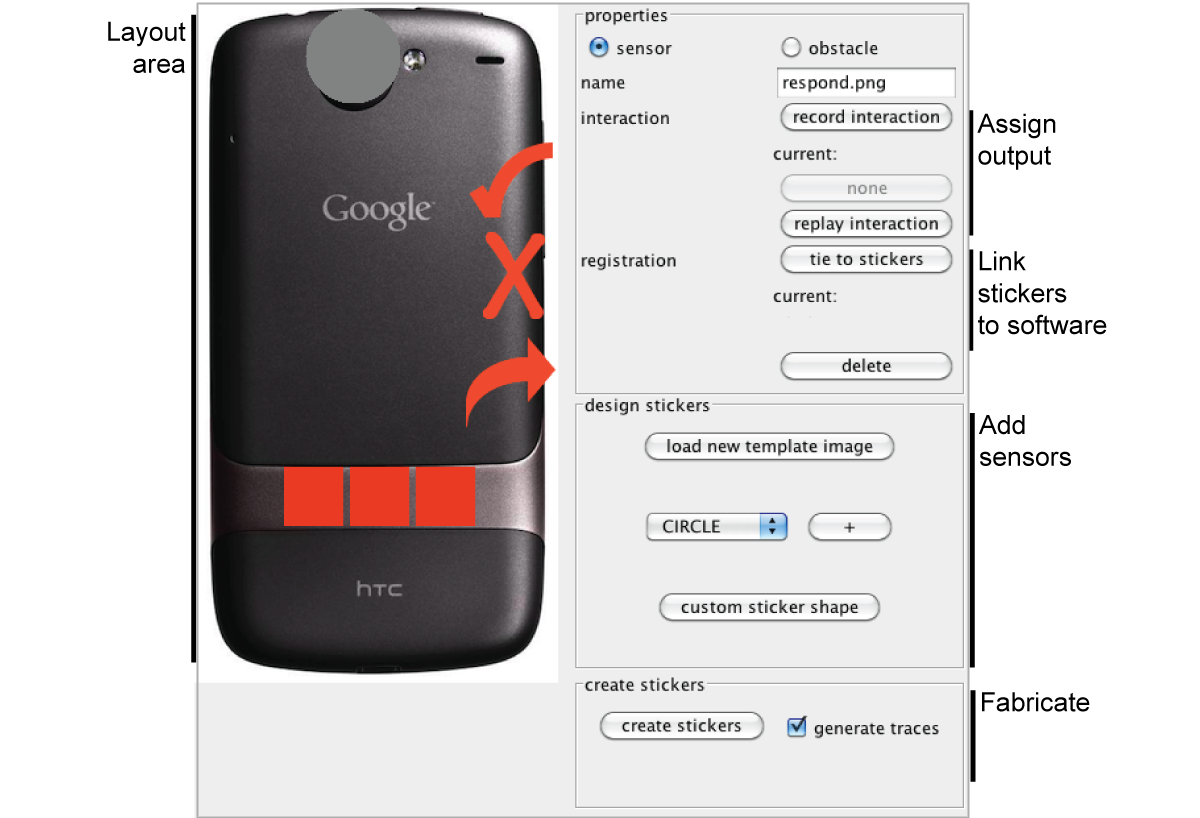
\includegraphics[width=3.5in]{figures/midas/ui.png}
\caption{Midas's sensor editor takes its cues from GUI editors: designers first lay out sensing areas through direct manipulation; they later define interactions for each sensor using a property inspector.} 
\label{fig:midas-editor}
\end{figure}


        \subsubsection{Fabricating and Applying Flexible Sensors}
Once users complete a layout, clicking the ``Create Stickers''
button generates fabrication files. First, certain components
are automatically split into multiple sensing pads. For instance,
a slider can generate four interdigitated pads (Figure \ref{fig:midas-templates}, third template) for continuous finger tracking, while
2D pads result in two separate layers of triangular pads (Figure
\ref{fig:midas-layering}). Second, Midas generates conductive traces that will
connect each of the pads to Midas's touch controller. An additional mask file, to be fabricated in vinyl, includes cutouts
of only the sensor shapes: it will cover the traces both for aesthetic
reasons and to prevent stray touch events. Midas's connection
routing determines the exact position of each touch
area. Should the user want to experiment with positioning,
Midas can also skip routing and only generate individual
touch pads. However, the user must then manually connect
wires to each sensor and register the sensor in the interface.

The pad creation and routing step generates a set of graphics
files (in SVG format) and an instruction sheet (in HTML)
which appears in the user's browser (see Figure \ref{fig:midas-instructions}). This sheet
contains step-by-step instructions describing how to fabricate
the generated files. For our implementation, instructions include
which SVG files to cut in which material and how to
transfer the cut designs to the prototype object.

In our phone example, the designer generates one SVG file
for the touch areas and one to mask the traces, which prevents
stray touch events. Following the generated instruction
web page, she feeds copper foil into her vinyl cutter and cuts
the corresponding SVG file. She then substitutes a vinyl roll
and cuts a mask layer. As both materials have adhesive backing,
she sticks the copper and vinyl layers onto the phone
she wishes to modify. Once the adhesive layers are applied,
she tapes the end of the routed traces to the Midas hardware,
which is plugged into her computer via USB. Since the design
files for her prototype are digital, she also sends them to
colleagues in another office for a second, remote test. With
the design files and a vinyl cutter, her colleagues can then
recreate a working Midas prototype.

\begin{figure}[t!]
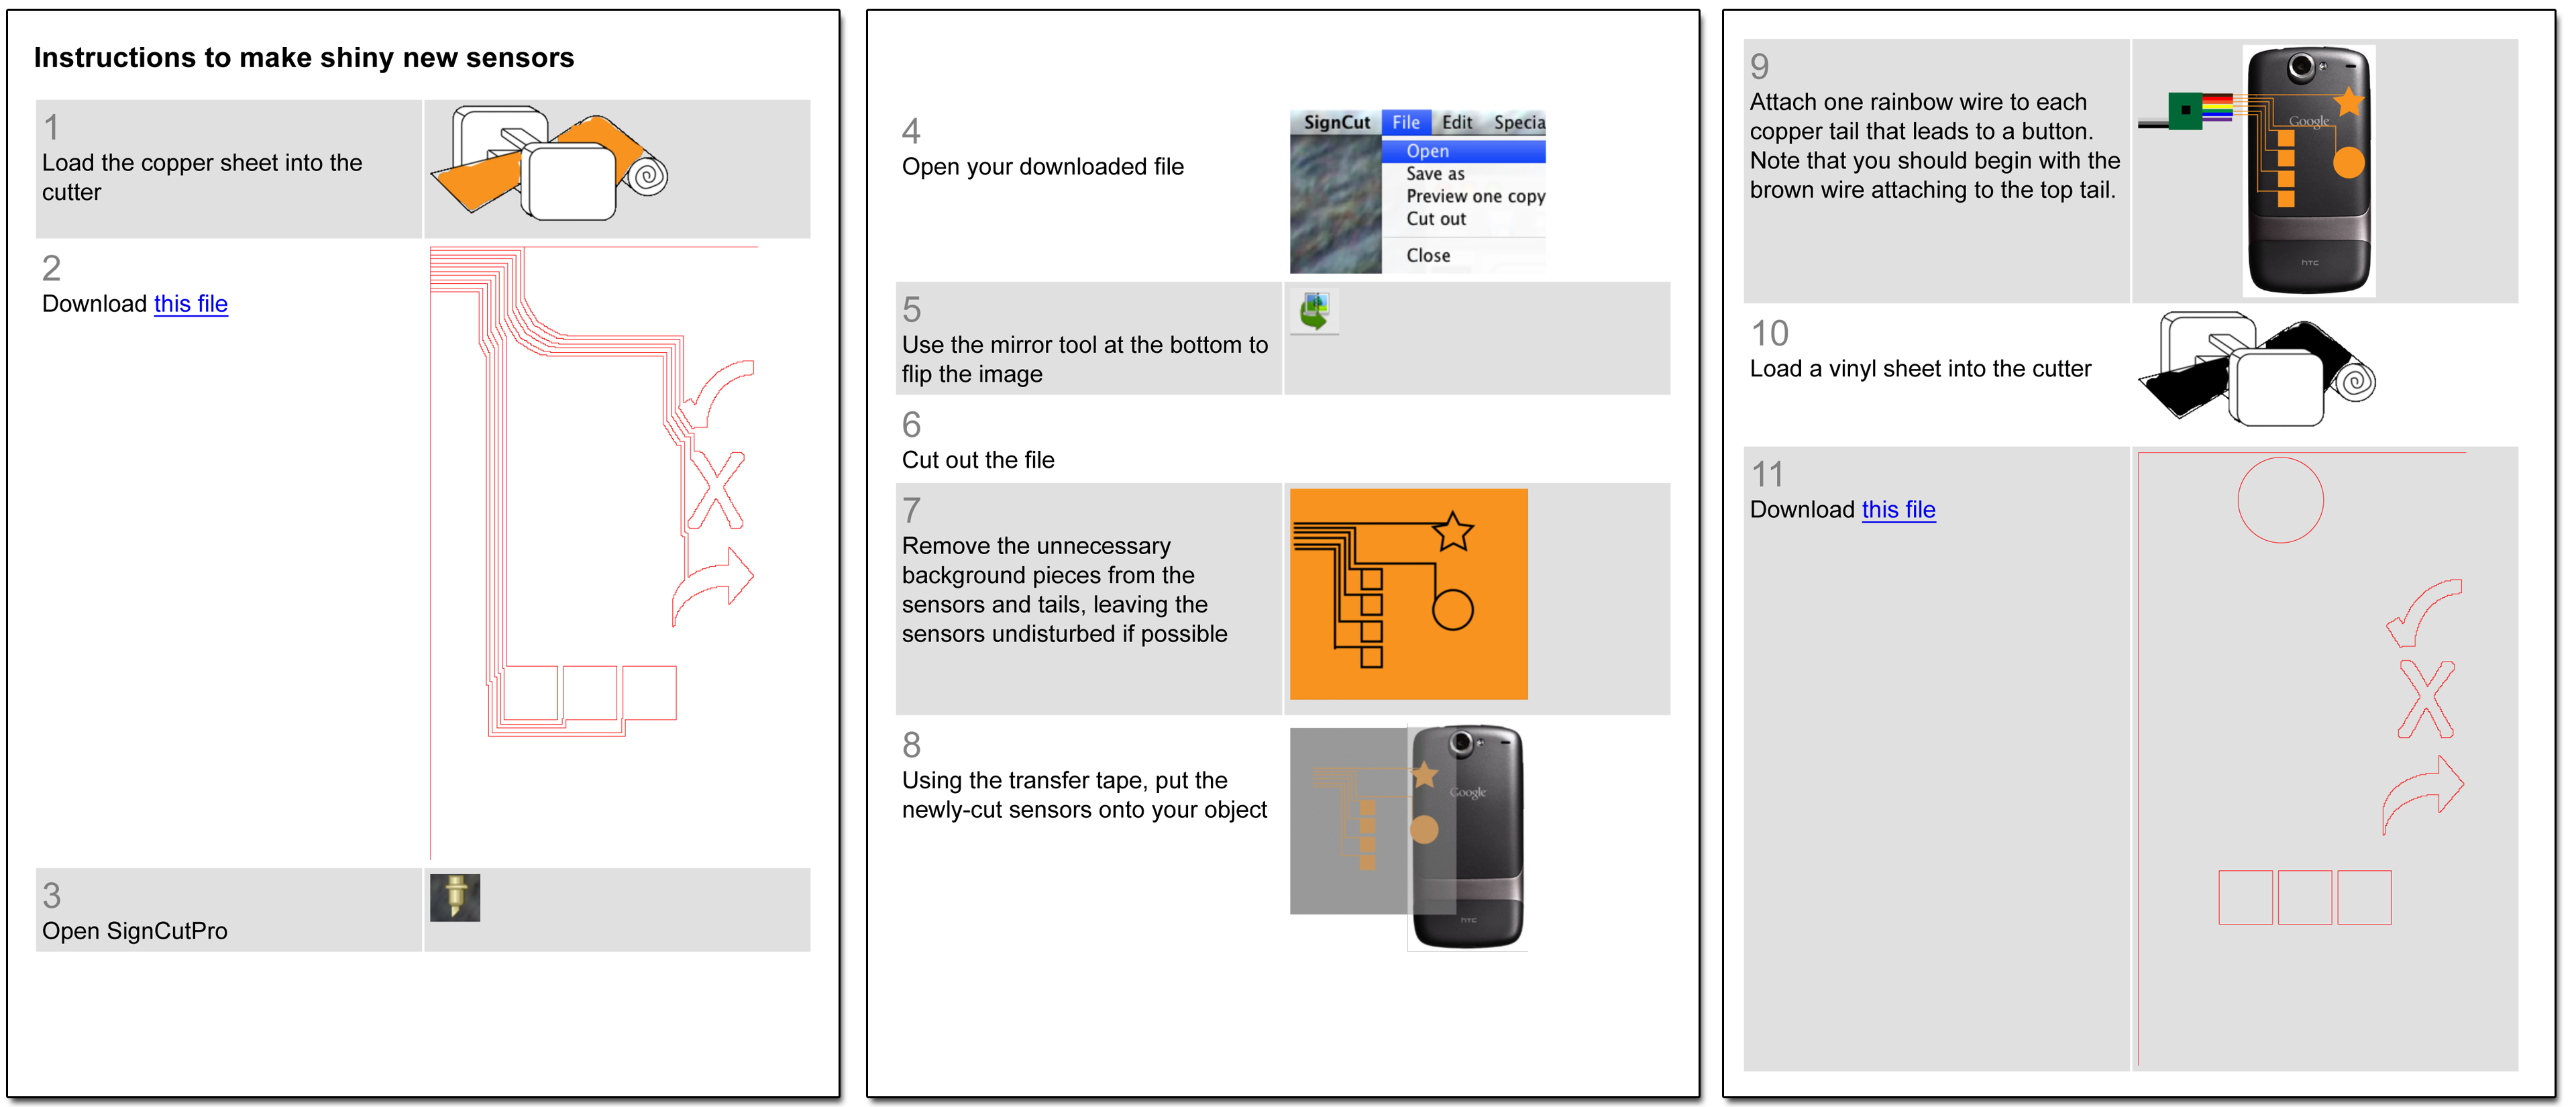
\includegraphics[width=\textwidth]{figures/midas/instructions.png}
\caption{Auto-generated step-by-step instructions in HTML format lead the user through the fabrication and assembly process. Relevant design files are hyperlinked to specific steps; instructions also include general help on processes, e.g., how to use transfer tape to apply a sensor onto an object.} 
\label{fig:midas-instructions}
\end{figure}

        \subsubsection{Connecting Hardware to Software}
Midas senses touch events with a dedicated touch controller
circuit board. Users do not have to program or assemble any
electronics---they may treat the entire setup as a prototyping
“dongle”. Users do have to connect the end of the traces to
the controller's rainbow ribbon cable, either by taping the
cable leads onto copper traces or by soldering them.

To complete a prototype, users return to the sensor editor. In
many toolkits, mapping hardware components to named objects
in software can be error-prone---it is easy to swap wires
or connect to an incorrect pin. If the user prints a fully-routed
design, Midas generates instructions for aligning touch areas
with specific ribbon cable colors. If the user decides to wire 
the design herself, this mapping has to be authored. Midas
uses guided demonstration to assist with this process. For
buttons, the user selects an input element in the UI and clicks
the ``Tie to Stickers'' button; next she touches the corresponding
copper sensor. Midas listens for status change events and
automatically assigns hardware pins. Midas registers sliders
similarly: users are asked to swipe a finger along the slider.

Midas's editor interface displays incoming touch data visually,
re-coloring touched sensors in pink on the sensor editor,
to aid the user in debugging. If something goes wrong during
the connection stage, it is apparent to the user. Midas
also reads the data stream for common errors. If it detects
that two wires may be too close together and triggering each
other, or that there may be a faulty connection from a wire
to the board, that information is displayed to the user in a
connection status area.

\begin{figure}[t!]
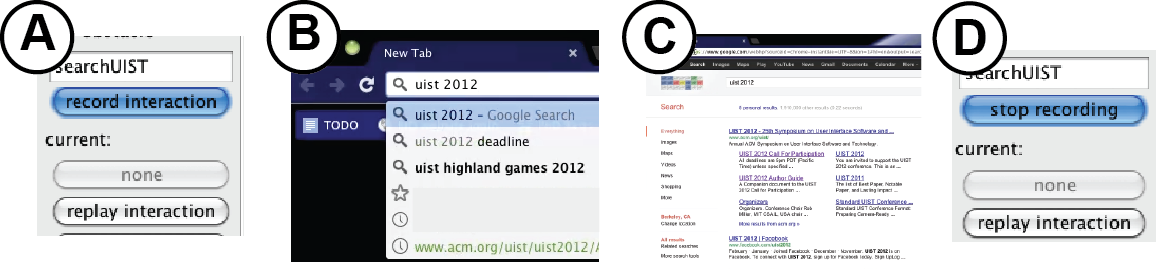
\includegraphics[width=\textwidth]{figures/midas/demonstrate.png}
\caption{Users start to record GUI interactions in the sensor editor (A); they can for example activate the browser, enter text (B), and click on a search result (C), before concluding the recording (D). This sequence of actions can then be triggered by a touch event.} 
\label{fig:midas-demonstrate}
\end{figure}

        \subsubsection{Adding Interactivity}
Designers have two options for authoring interactivity: record-and-replay
of mouse and keyboard events (a strategy adopted
from BOXES \cite{hudson-boxes} and Exemplar \cite{hartmann-exemplar}), or touch event output
to control applications via WebSockets. To record and replay
interactions, designers select a sensor in the editor, then click
on the ``Record Interaction'' button. They can then control any
open application (e.g., start or stop a media player application,
or drag a volume slider). Midas records the generated
keyboard and mouse events and can replay them later in response
to touch input (Figure \ref{fig:midas-demonstrate}).

The types of desktop UI actions that can be executed depend
on the button type. Individual buttons can be tied to an interaction
script, a sequence of keyboard and mouse events
recorded by the user. Sliders are linked to exactly one horizontal
or vertical line on the screen to be controlled by clicks
along its length. 2D pads can control a 2D area on the screen
analogous to a slider area. For sliders and pads, the user must
capture the location on the screen that she wishes to control
with the slider or pad. This is done by clicking at each end
of the slider or in opposite corners of the pad, guided by Midas
prompts. As the user adjusts the sensitivity (number of
discrete buttons) of the slider or pad to be printed, the interaction
with the captured on-screen slider or pad becomes
more fine-grained, also.

Record-and-replay does not require programming, but it is
brittle; changes in application layout or response latency can
break a recorded sequence. To let users author more robust
interactions, Midas uses WebSockets to send touch events
over the Internet. This requires programming, but WebSockets
enable designers to work in the languages many are most
familiar with: HTML and JavaScript.

In our phone example, the designer chooses WebSockets as
she wants to demonstrate how touch events can control a mobile
email application. She creates a mockup in HTML and
writes JavaScript functions to receive touch events.

\section{Implementation}

In this section, we describe the Midas design tool, the hardware it uses for sensing, and fabrication techniques for manufacturing compatible sensors. 

    \subsection{The Midas CAD tool}
    
    We discuss the key parts of the Midas CAD tool: generating sensor pads and routing pads to the touch controller.

        \subsubsection{Generating Sensor Pads}

The Midas sensor editor supports four types of touch sensors:
discrete buttons, two types of 1D sliders, and 2D pads. The
resolution of pads and segmented sliders can be set through a
parameter in the sensor editor. The current editor is written in
Java using the Swing GUI Toolkit. Figure \ref{fig:midas-templates} shows example
templates for each sensor type. The two types of sliders are
based on different sensing approaches. The first, segmented
slider, is made up of individual rectangular touch segments.
Users specify how many segments the slider has. Continuous
sliders offer finer resolution, but require a different detection
approach. We use Bigelow's design of interdigitated electrodes
\cite{bigelow-interdigitated}. In this design, as a finger slides across the pads,
the surface area of the pads underneath the finger changes as
pad digits get smaller or larger. Because capacitance is proportional
to contact surface area, the measured capacitance of
each segment changes during the finger's slide. Though finer
in resolution, only one such slider is supported by our current
sensing hardware. Increasing the number of supported
sliders is possible with additional engineering effort.


\begin{figure}
\centering
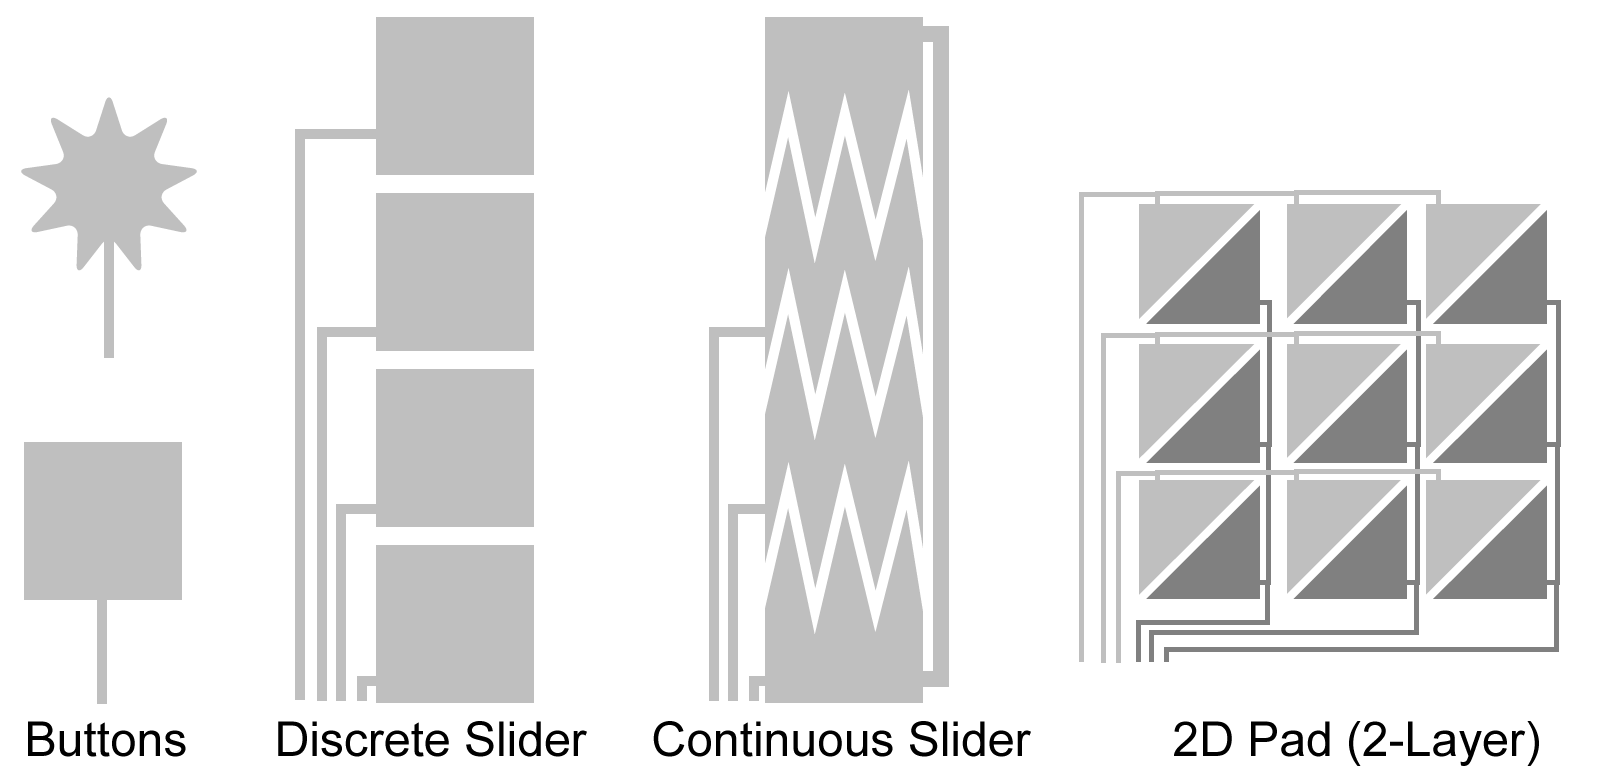
\includegraphics[width=3.25in]{figures/midas/pad-templates.png}
\caption{Midas can generate four different types of sensors: discrete buttons, discrete sliders, continuous sliders, and 2D pads. The pad uses row-column scanning and requires multi-layer construction because traces cross.} 
\label{fig:midas-templates}
\end{figure}

\begin{figure}
\centering
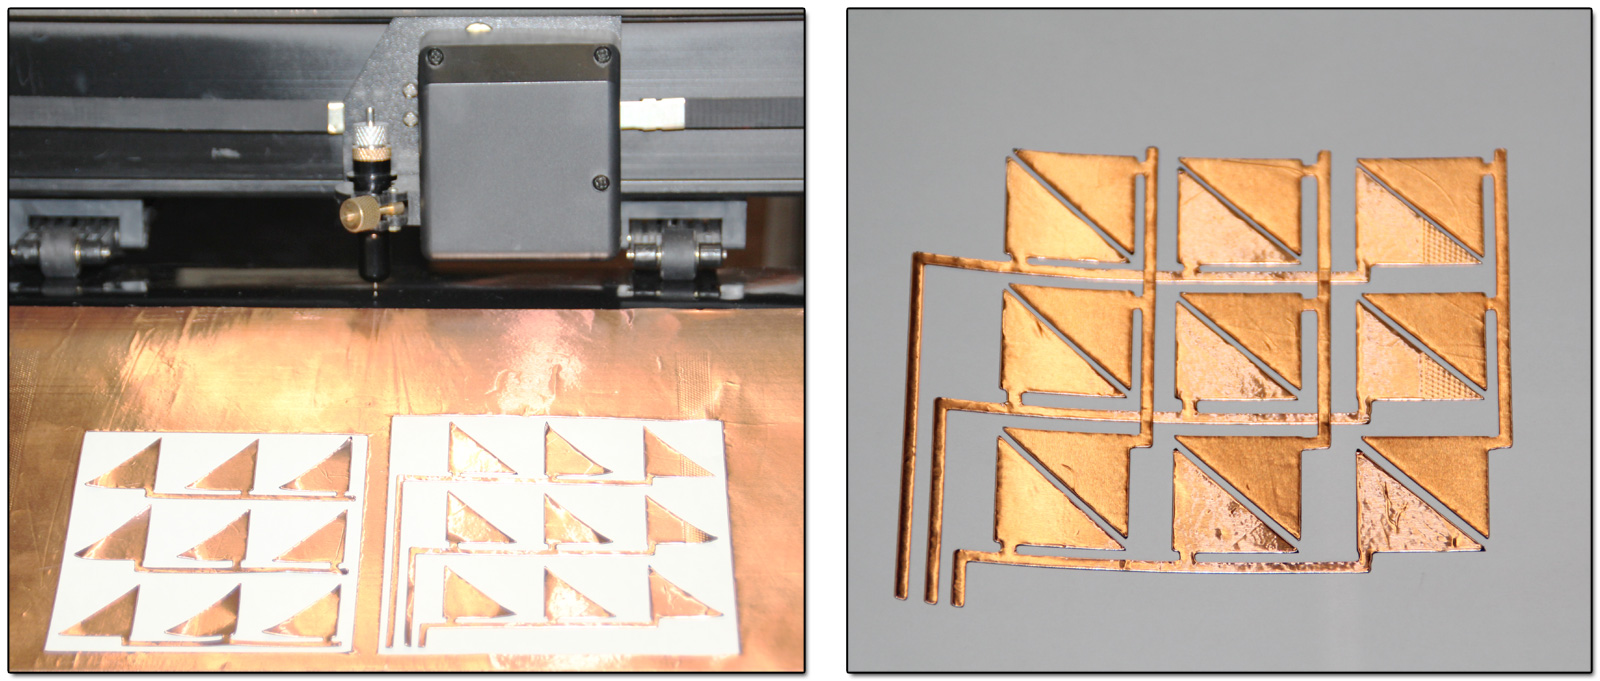
\includegraphics[width=3.25in]{figures/midas/2dgrid.jpg}
\caption{2D pad sensors are fabricated in two different layers that are then superimposed. Because each copper layer has a vinyl backing, no other inter-layer masking is required.} 
\label{fig:midas-layering}
\end{figure}

2D pads use row-column scanning to reduce connecting traces.
For example, a $5 × 5$ array requires $25$ individual traces, but
only $5 + 5 = 10$ row-column traces. This design requires a
dual-layer construction where horizontal traces are isolated
from vertical traces. We use copper foil applied to vinyl foil
in our cutter, so each layer already has an insulating substrate.
Designers thus first apply the bottom conductive layer,
then place the top layer directly over it (see Figure \ref{fig:midas-layering}).
To create a mask layer that covers the topmost copper traces,
we generate a design file containing pads from all layers, but
no traces. This layer is cut in vinyl. While for other layers
designers transfer the pads and traces, for the mask layer they
peel and transfer the surrounding “background” shape with
sensors and obstacles cut out (see Figure \ref{fig:midas-pinball}, left).


        \subsubsection{Routing Pads to the Touch Controller}
Midas employs an auto-routing algorithm to generate conductive
traces connecting electrodes to the Midas touch controller.
User-defined obstacles are avoided. We implement
Lee's breadth-first maze routing algorithm for single layer
paths \cite{lee-maze} (see Figure \ref{fig:midas-routing}). This algorithm selects a source and target (the source is the trace anchor for connecting to the microcontroller, the target is all pixels on the perimeter of the sensor). Then, beginning at the source, floods the grid by marking each viable pixel---i.e., pixels which are not on obstacles and which will not touch other sensors---with its distance from the source. When any of the target locations are reached, the algorithm traces back through the marked pixels, maintaining straight traces as much as possible, and generating a trace along the path selected. For 2D pads, we perform two independent routings:
one for the row layer and one for the column layer. Our
current algorithm does not generate vias (connections between
different conductive layers). When auto-routing fails,
we employ an iterative search by adjusting the position where
traces connect to sensor pads, routing the sensors in a different
order, or moving the position where target traces connect
to the touch controller. In our experience, this basic routing
algorithm has performed adequately, though there are designs
that cannot be successfully routed. For such cases, the
algorithm could be replaced with more sophisticated routing
techniques that include user input, though such techniques
require that the user has a correct mental model of the routing
process.

Midas currently offers generic suggestions when routing fails,
e.g.: “Sensor reply may be too close to sensor delete. Try
moving sensors away from the edge and each other.”

\begin{figure}[t]
\centering
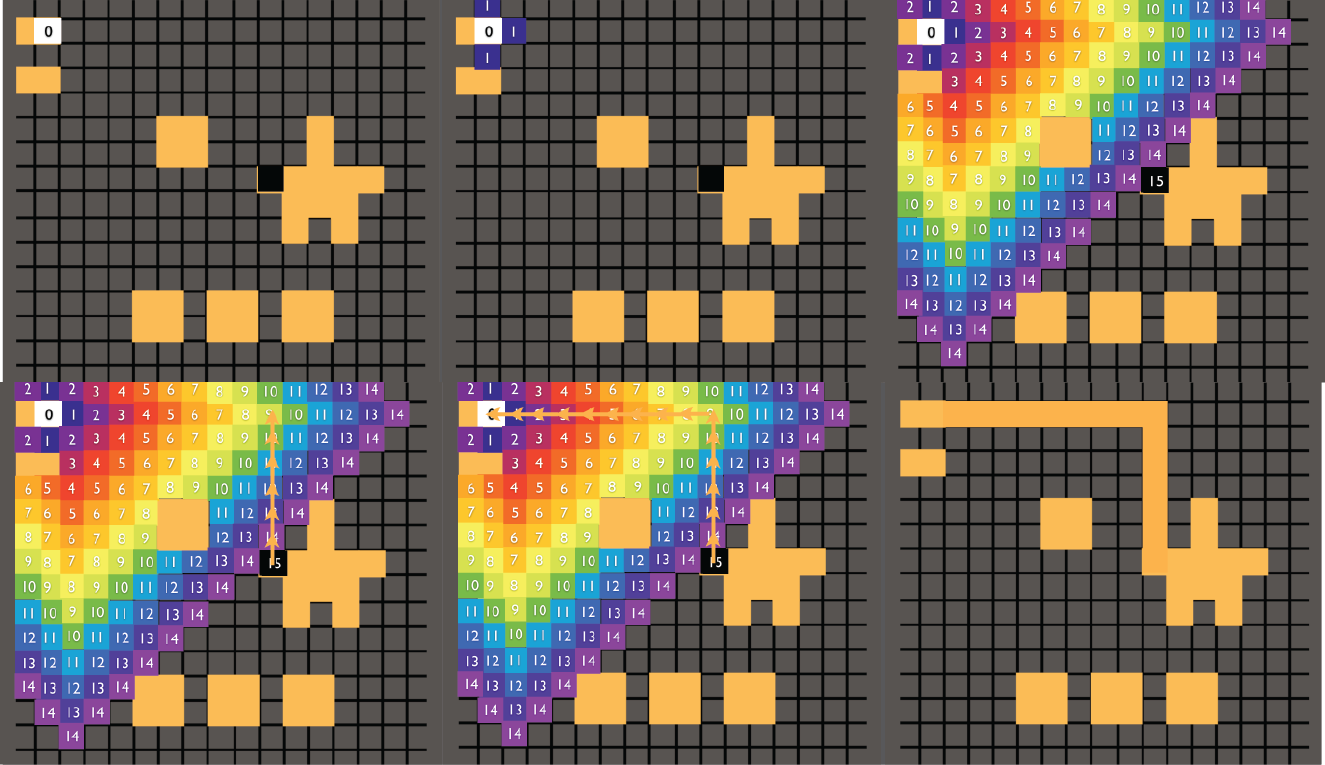
\includegraphics[width=5in]{figures/midas/routing.png}
\caption{The Midas routing algorithm, based on Lee's \cite{lee-maze}, first selects a source and target point. It then floods the grid, beginning at the source, marking each viable ``pixel'' as one further than its pre-marked neighbor. Once the target has been reached, the algorithm traces back through the marked pixels (we selected to make vertical moves before horizontal) to the source and creates a trace.} 
\label{fig:midas-routing}
\end{figure}


    \subsection{The Midas Hardware}

We discuss the components of the Midas hardware: the mechanism of capacitive touch sensing and the fabrication of compatible sensor pads. We also describe how the sensed and digitized signal is used to design interactions.

    \subsubsection{Sensing Mechanism}

        Midas relies on capacitive touch sensing. The Midas touch controller (Figure~\ref{fig:midas-microcontroller}) is based on an Atmel microcontroller board~\cite{teensy} and capacitive sensing chips from Quantum (QT1106) and Freescale (MPR121) Semiconductors. For discrete inputs, both chips rely on charge-transfer sensing using single-wire electrodes: the electrodes are part of a simple RC circuit in which an output pin is set high, and time is measured until an input pin also reads high. This time is proportional to the capacitance of the circuit: when a person touches an electrode, the circuit capacitance and the charge transfer time both increase. The Quantum chip also implements Bigelow's design to extract continuous position readings from interdigitated electrodes by interpolating based on relative capacitance between neighboring pads~\cite{bigelow-interdigitated}. The microcontroller runs software written in embedded C to interface with the sensor chips and communicates touch data to a connected computer over USB. It recalibrates the touch sensing chips periodically to ensure floating sensor values do not lead to erroneous touch readings.
        
        Our new Midas touch controller uses an Adafruit Blufruit microcontroller with Bluetooth compatibility. It does not implement Bigelow's interdigitated sensing but could do so in the future; for discrete sensing it leverages the Arduino CapSense library\footnote{\url{playground.arduino.cc/Main/CapacitiveSensor?from=Main.CapSense}} which uses two-wire electrodes; it determines the capacitance by timing the charge transfer time between the pins. The new board design also has sturdy milled connection pads to attach to traces; these can be attached using Z-axis conductive tape (e.g., 3M's Z-Axis Conductive Tape 9703). This board transmits sensed readings directly to a phone over a Bluetooth connection.
        
        \begin{figure}[b]
        \centering
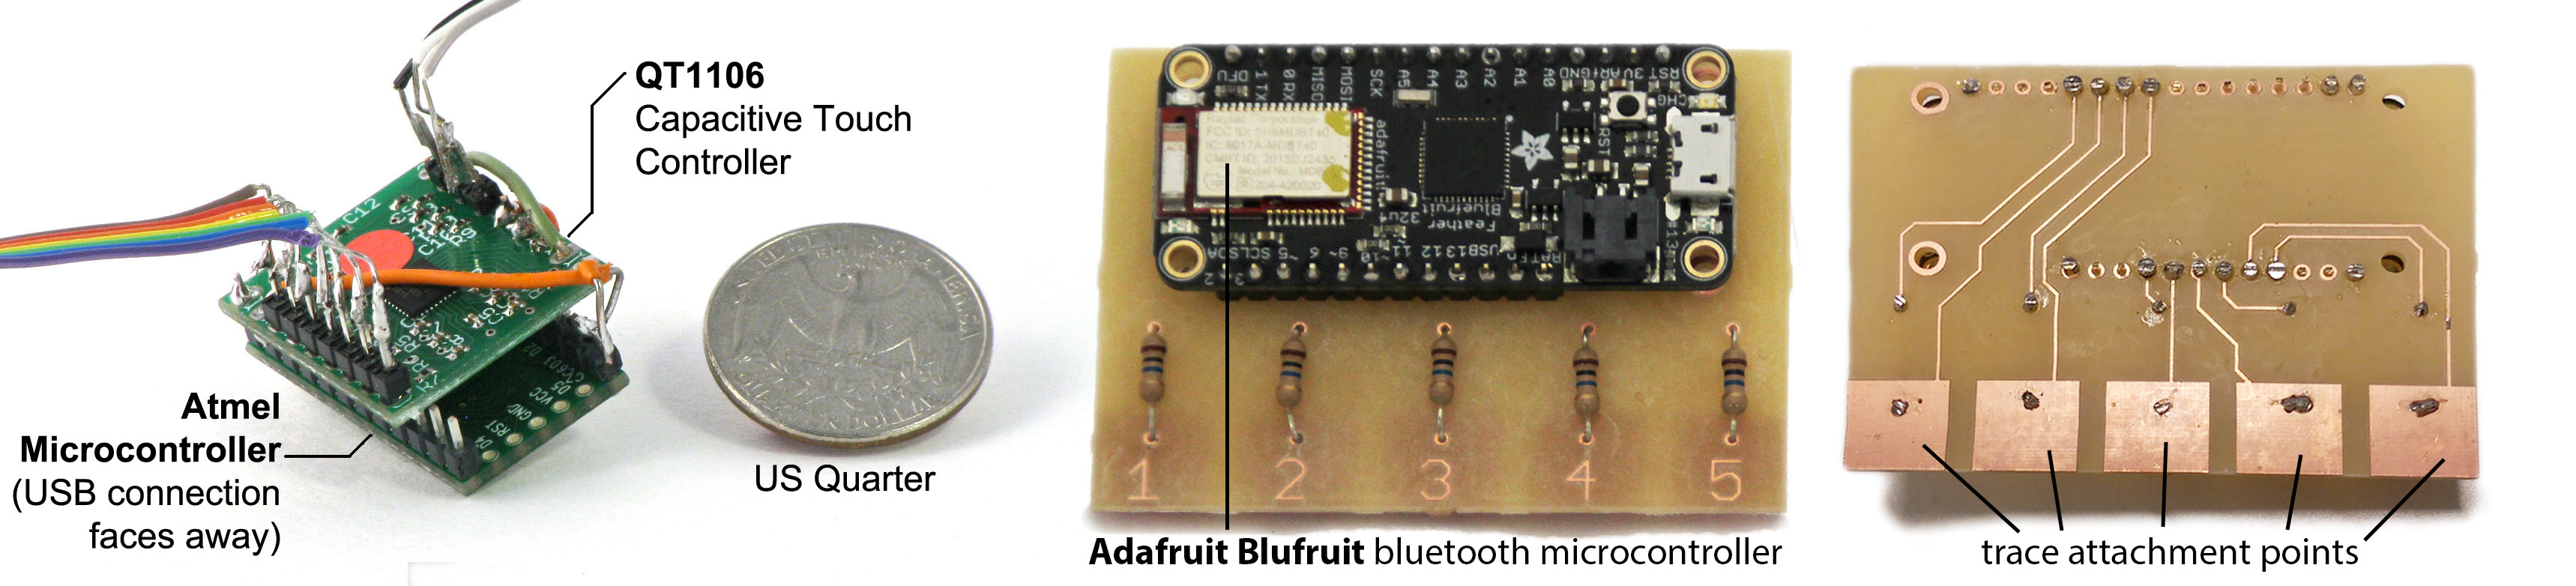
\includegraphics[width=6in]{figures/midas/microcontrollerz.jpg}
\caption{The original Midas touch controller board (left) uses a commercial capacitive charge transfer detection chip to sense touch events. Events are relayed to a computer via a mini USB connection on the back. The ribbon cables are used to connect to the end of routed traces. The new board (right) uses an Arduino touch sensing library and a Bluetooth-compatible microcontroller for wireless data transmission and sensing. A US quarter is shown as a size reference.} 
\label{fig:midas-microcontroller}
\end{figure}

    \subsubsection{Fabrication}
    
    \begin{figure}[b]
    \centering
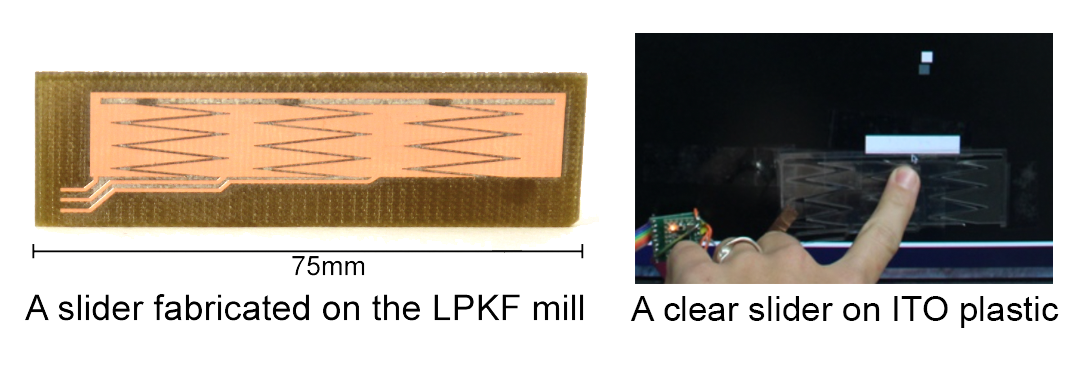
\includegraphics[width=\textwidth]{figures/midas/otheroptions.png}
\caption{Two example touch sensors fabricated with alternative processes: left, a hard sensor created on a circuit board mill. Right, a sensor cut from Indium Tin Oxide-coated transparent plastic..} 
\label{fig:midas-dimatix}
\end{figure}

Midas generates vector graphics files in SVG format for the
electrode and mask layers. These files can be used to control
digital fabrication processes. Our prototype currently
cuts conductive, adhesive-backed copper foil on a commercial
vinyl cutter---a plotter with a cutting knife instead of a
pen. This medium has multiple advantages. First, it is cost-effective
and readily available: vinyl cutters are in the same
price range as laser printers (ours, a tabletop model with a
$35cm$ bed, cost \$$200$); and copper foil costs a few dollars
per foot. Second, copper has excellent conductivity. Third
flexible, adhesive foil is easy to apply to non-planar surfaces.
However, there are important drawbacks as well. Most importantly,
the cutting process and manual weeding (removing
background material) determines a minimum feature size
for traces. Thin geometric features can also break during
transfer, and the weeding process can be tedious and time-consuming.
We found the most success adhering
the copper sheets to vinyl sheets and cutting both layers at
once. This setup has the added benefit of allowing designers
to prototype touch interactions on conductive surfaces (e.g.,
aluminum casing) as vinyl is an excellent insulator.
Alternative fabrication processes may be preferable to copper
foil cutting when higher precision or durability is required.
Three promising approaches are circuit board milling, which
can produce smaller features but is limited to rigid boards; cutting from Indium Tin Oxide (ITO)-coated plastic, which allows for transparent sensors but is not self-adhesive and is less flexible than vinyl;
and conductive inkjet printing, which can produce the smallest
features, but is not yet available to many end users. As
a proof of concept, we produced a touch sensor on an LPKF
circuit board milling machine, and one on a Silhouette Cameo paper cutter (see Figure \ref{fig:midas-dimatix}).

\subsubsection{Debugging}

Midas offers basic debugging support. The interface displays incoming touch information from the microcontroller, highlighting activated sensors.  We have also implemented basic regular expression filtering on the touch stream to help the user identify potential problems.  A time-stamp and code representing each touch event is stored in a stream.  When a sensor is ``stuck on'' for more than $10$ seconds, Midas reports that that sensor may be touching another wire.  When a touch sensor ``flickers'' on and off more than twice within $500ms$, Midas suggests that there may be a faulty connection from that sensor to the microcontroller.

\subsection{Event Output}
Once the user has assigned interface scripts to sensors, Midas listens for events from the touch controller. When a touch event matches the key of a saved interaction, that interaction's associated script is executed.

\subsubsection{Record-And-Replay}

In record-and-replay, the user selects a sensor and records a sequence of mouse and keyboard actions that should be played back when the sensor is touched. Early prototypes of Midas used Sikuli for this purpose---a scripting language based on computer vision analysis of screenshots~\cite{yeh-sikuli}. While more robust than hardcoded click locations, Sikuli was designed for automation scripts rather than interactive control, and the latency of invoking and executing scripts was too high. Our current prototype uses the Java Robot API~\cite{robots} to captures and replay both mouse clicks and keyboard events. We share this approach with the BOXES system~\cite{hudson-boxes}.

\begin{figure}[b]
\centering
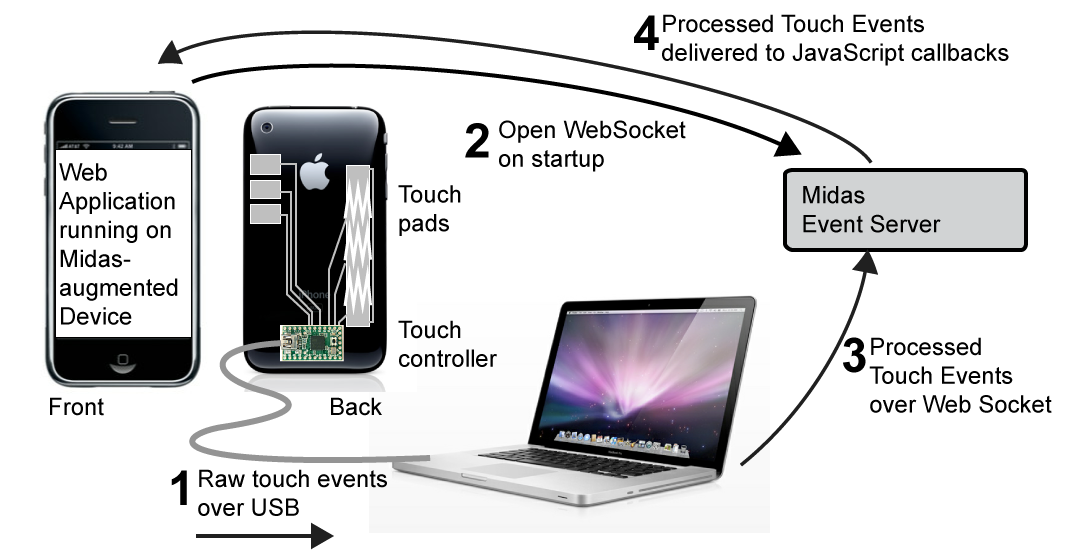
\includegraphics[width=3.25in]{figures/midas/socket-events.png}
\caption{Midas's socket event output enables designers with programming knowledge to create web applications in HTML and JavaScript that react to touch input outside the screen area of a phone or tablet.} 
\label{fig:midas-socket}
\end{figure}

\subsubsection{WebSocket Communication with Web Applications}

Record-and-replay is restricted to applications running on the same machine as the sensor editor, and it is limited to mouse and keyboard event injection. To surmount this limitation, Midas can also export touch events to remote clients via a built-in server using the WebSockets API. For example, an application running on a smart phone can open a WebSocket connection to Midas and receive a callback for any Midas button, slider or pad event. The callback function receives an event object describing which sensor changed state, and the value of the new state (e.g., on/off, or slider value).

Our WebSockets server is implemented in node.js using the socket.io library. We chose WebSockets because it offers full-duplex communication at low latencies, and, more importantly, is supported by modern web browsers. This means designers can author user interfaces that respond to Midas touch input in HTML and JavaScript. There are two main benefits to these technologies: (1) many designers are already familiar with them from web design; (2) developed interfaces can be deployed on any device with a compatible browser, even if that device does not offer a way to directly connect external hardware. For example, it is difficult to directly connect sensors to Apple's iPhone or iPad.

With our WebSockets architecture (Figure~\ref{fig:midas-socket}), designers open a browser and enter the URL of an HTML file they have placed in the Midas server directory. This file opens a socket connection from the phone browser to Midas. When Midas receives events from the touch controller, it forwards them to the client, which can then show visual feedback.

\subsection{Bluetooth}

Our new touch controller leverages Bluetooth for communication. The detected data are streamed similarly to those in the WebSockets condition, however in this case they are transmitted via Bluetooth, and the receiving device must be paired to the controller.

\section{Evaluation}

    In order to demonstrate that Midas's sensing and fabrication technique fits our criteria of being a cheap, fast, and flexible method of prototyping, we elaborate on each of these criteria below.

    \subsection{Cost-Effective}
    
    Midas enables touch-sensitive prototyping for roughly the cost of a laser printer. The vinyl cutter used for the Midas project, a tabletop model with a $35cm$ bed, cost \$$200$. Copper foil costs a few dollars per foot.
    
    Alternatives to this fabrication method include cutting Indium Tin Oxide (ITO)-coated plastics, using silver ink in an inkjet printer, and fabrication using a circuitboard mill. ITO-coated plastics allow for transparent sensors; ITO costs roughly \$$.25/in^2$ and can be fabricated on an inexpensive paper cutter. Silver ink can be used in many existing inkjet printers, and costs roughly \$$1/mL$ or \$$2/ft^2$ of total coverage. Circuitboard milling has a high startup cost (a suitable machine can cost as little as \$$800$, and upwards beyond that), but the per-unit expense is low, about \$$17/ft^2$.
    
    On the sensor side, the full sensor setup we prototyped with cost \$$36$: \$$16$ for the Arduino Teensy microcontroller board, and \$$10$ for each of the capacitive sensing breakout boards. This cost could be reduced further with custom circuitboards (our setup was assembled from commercially-available boards for expediency), and the setup is can be easily detached from a prototype and reused in a new iteration or for a different project.
    
    \subsection{Fast}
    
    We did an informal first-use study, and it took all participants $<1$ hour to both receive training and create working media player peripherals with the system.
    
    We recruited three participants for this study. Two were graduate students at UC Berkeley (in Computer Science and Mechanical Engineering), and the third was a software engineer at a local technology company. All had some prior experience with prototyping and electronics.

        \subsubsection{Procedure}
Participants received a walkthrough of Midas including a simple record-and-replay task to launch a browser based on a single button input. Participants were then asked to design a physical control interface for a media player (iTunes). No other constraints were given as we wished to encourage exploration. Participants completed a post-task questionnaire with open-ended questions on interface usability and workflow utility.

    \subsubsection{Results}
All participants successfully designed media players (Figure~\ref{fig:midas-study1}). Participants commented positively on how Midas aided them with the task of physical construction---both by routing connections and through the generated instructions. Record-and-replay was easy to comprehend and effective for the given task. Though the task did not require programming, two participants expressed interest in receiving touch events in their own applications. We take this as corroboration for the utility of our WebSocket server. Participants additionally identified several areas for improvement (including more detailed instructions, additional help for auto-routing failures, and additional feedback for touch events), which are included in our most recent design revision, described above.

\begin{figure}[t]
\centering
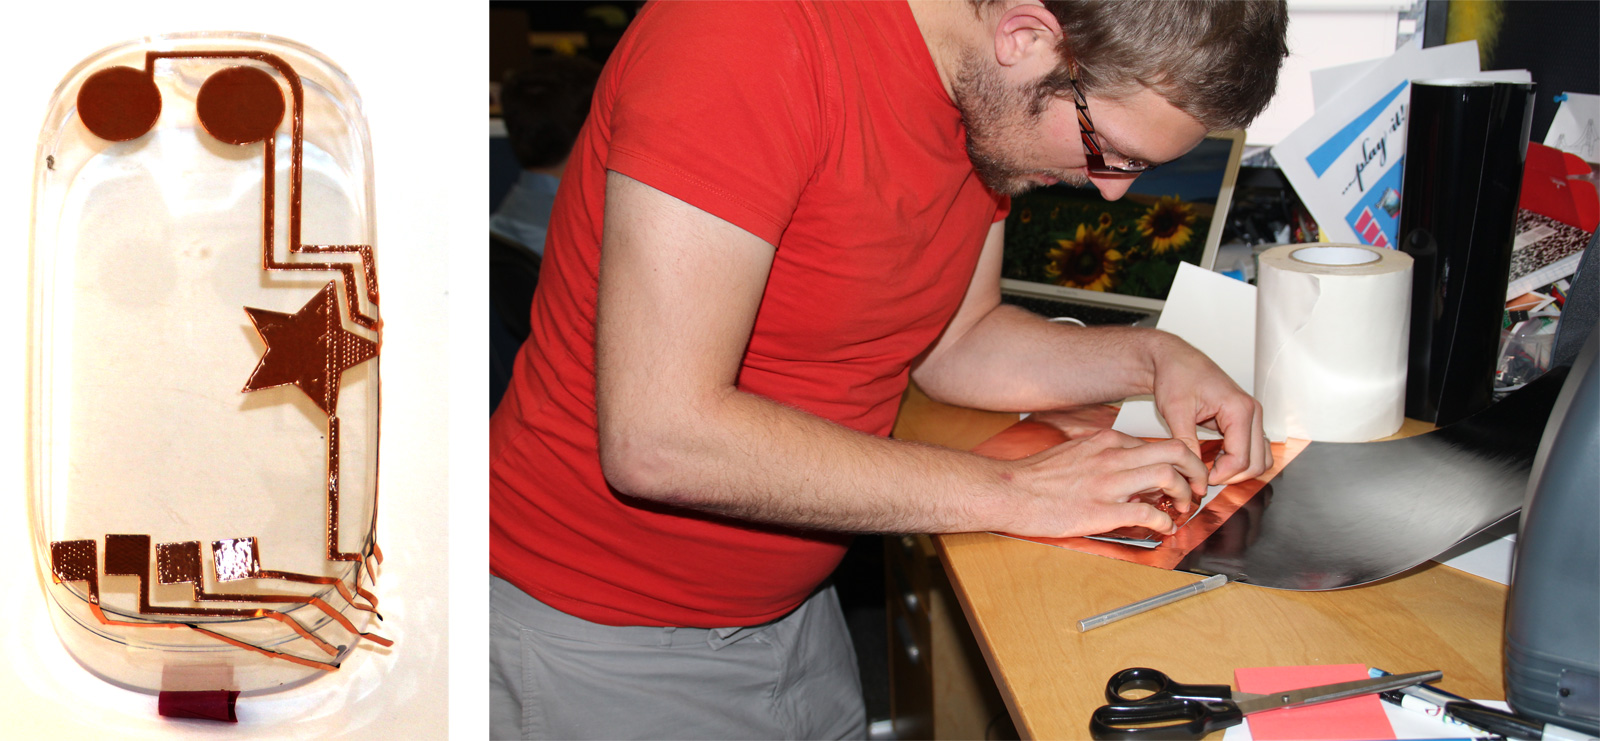
\includegraphics[width=3.25in]{figures/midas/study1.jpg}
\caption{A study participant's sensor layout for a PC media player peripheral.} 
\label{fig:midas-study1}
\end{figure}

    \subsection{Flexible}
    
    To demonstrate Midas's expressivity, we built several interactive systems that used all sensor types, and output using both WebSockets and record-and-replay.
    
        \subsubsection{Text Entry}
Wobrrock's EdgeWrite~\cite{wobbrock-edgewrite} is a unistroke text entry technique based on activating a series of corner points of a rectangle. Wobbrock demonstrated that this technique can be implemented using four discrete capacitive touch sensors~\cite{edgewrite-cap}. We cut four discrete buttons and a mask with Midas, attached them to the back of a smartphone, and implemented the EdgeWrite recognition algorithm in JavaScript (Figure~\ref{fig:midas-edgewrite}). Using socket events, we demonstrated how EdgeWrite can be used to enter text on the back of a mobile device, leaving the screen unobstructed. The implementation is functional, though latency for detecting single button presses was higher than expected (\textgreater 100ms). We plan to investigate ways to increase responsiveness in future work.

\begin{figure}[t]
\centering
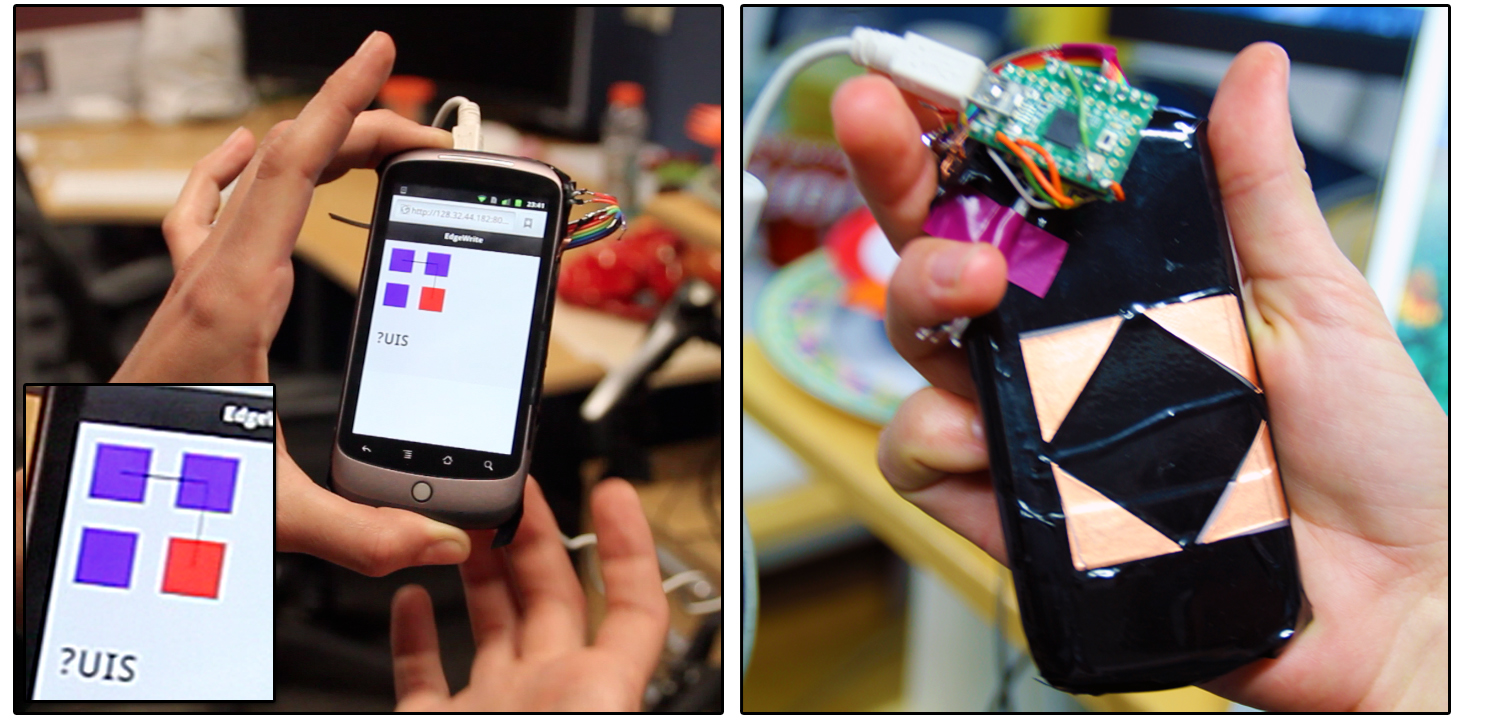
\includegraphics[width=3.25in]{figures/midas/edgewrite.jpg}
\caption{We implemented Wobbrock's Edgewrite on the back of a cell phone using a 2x2 pad and WebSocket events sent to a web page.} 
\label{fig:midas-edgewrite}
\end{figure}

        \subsubsection{Game Controller}
To test the responsiveness of Midas's continuous slider, we created a simple game controller for Breakout, in which players horizontally position a paddle to bounce a ball into layers of blocks (see Figure \ref{fig:midas-dimatix}). In less than fifteen minutes, we attached the slider and mapped slider position to paddle position using record-and-replay.
The slider is more responsive than individual buttons, and we were able to control the paddle accurately enough for gameplay.  The slider's response is non-linear across certain regions, however. Accounting for this is left to future work; our instinct says that it may be caused by electromagnetic interference from the thin traces and sharp right angles in the design.

We fabricated two versions of this game controller: one from a circuitboard milled slider, and a second from Indium Tin Oxide (ITO)-coated transparent plastic. This underscores the point that only the conductivity of the material is important; whether it is flexible/rigid or opaque/transparent has no bearing on the functionality.

        \subsubsection{Music Postcard}
At a recent media festival, a promotional poster printed with conductive ink enabled passersby to select and play music from a number of artists by touching corresponding areas on the poster~\cite{paperposter}. We implemented a postcard-sized version of this poster (Figure ~\ref{fig:midas-poster}).  We scaled back the size to conserve resources; large designs are possible and only restricted by the cutter's bed width. Our version uses six discrete buttons and one continuous slider to control playback and volume of music clips on a desktop computer. We again cut a vinyl mask layer to prevent stray touch events. We used Midas's record-and-replay function to remote control the iTunes music player.

\begin{figure}[t]
\centering
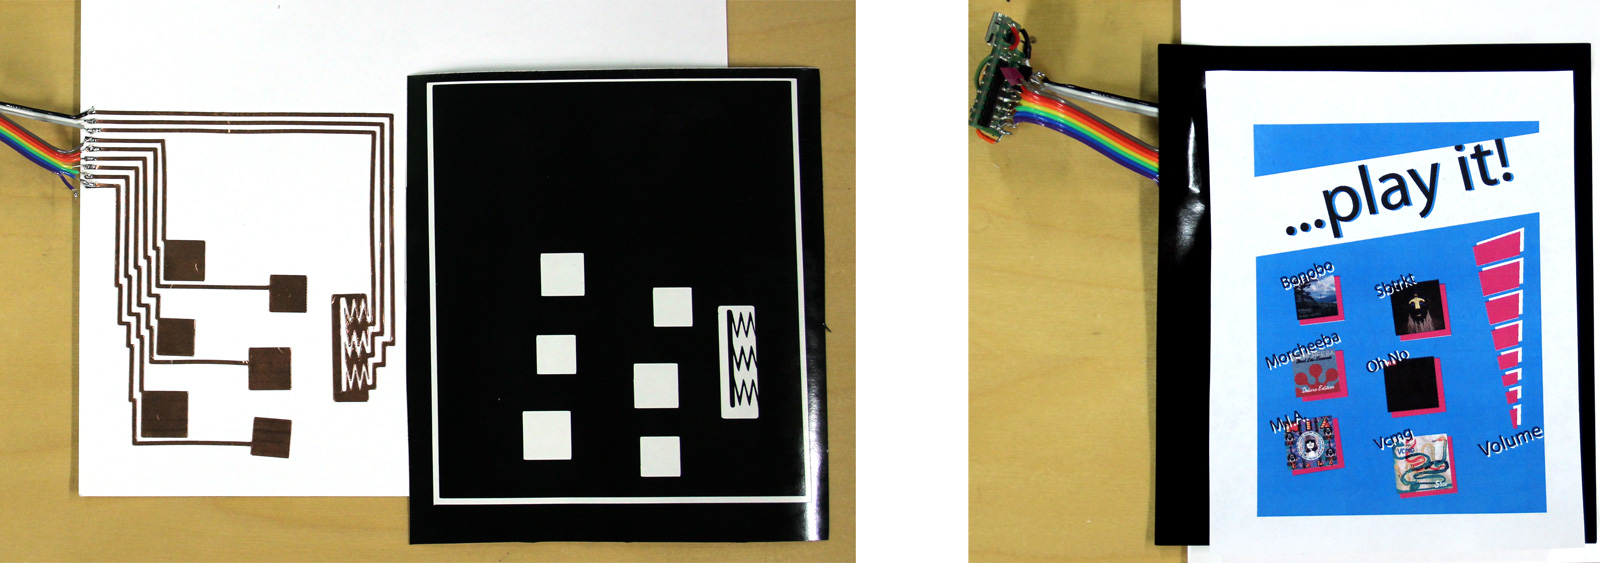
\includegraphics[width=3.25in]{figures/midas/poster3.jpg}
\caption{Our music postcard lets users sample tracks by different artists. Left: Circuit and mask layer; Right: assembled postcard.} 
\label{fig:midas-poster}
\end{figure}

        \subsubsection{Papercraft Pinball Machine}
Papercraft is the art of cutting and folding paper into 3D models. To demonstrate how Midas can be used for attaching sensors to more complex 3D shapes, 
%, and there are many popular templates for this hobby. Using this art, 
we created a papercraft pinball machine which can control a pinball game on a laptop. First we downloaded a template design for a pinball machine \cite{indianajones}, cut it out, and assembled it.  We then loaded the already-flattened template model into Midas's 2D editor interface and defined the negative space around the model as a routing obstacle (Figure ~\ref{fig:midas-pinball}). This guaranteed that all trace routing would be on the surface of the model. After attaching the two buttons for the bumpers and a continuous slider for ball release control, we used record and replay to control a desktop pinball game.

\begin{figure}
\centering
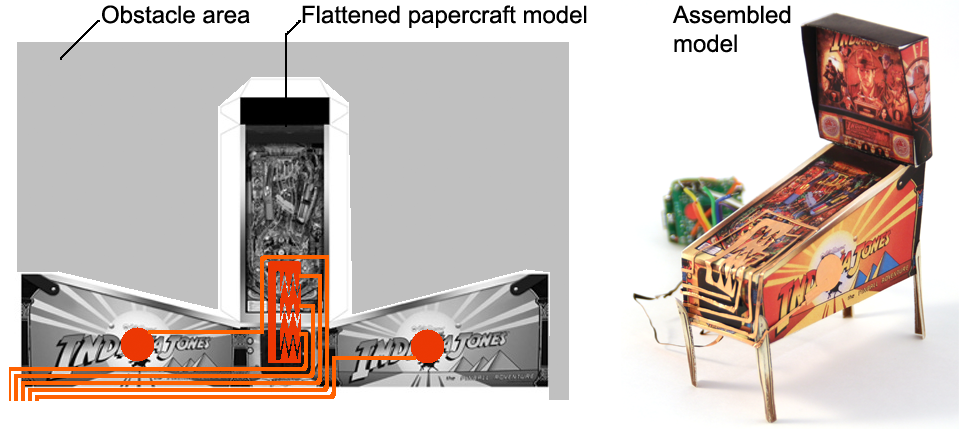
\includegraphics[width=3.25in]{figures/midas/pinball-horizontal.png}
\caption{For our papercraft pinball machine, we defined the negative space in the template as an obstacle to restrict sensor routing.} 
\label{fig:midas-pinball}
\end{figure}


\section{Discussion}

    Midas, as one of the first fabrication papers in the HCI community, explored a variety of interesting challenges and opportunities around digital fabrication. It serves several purposes well, but there are limitations caused both by the fundamental approach and the particular engineering of our prototype.

    \subsection{Sweet Spots}
    
    Midas is well-suited to prototyping particular kinds of objects. It allows facile testing and iteration on unusual types of touch interactions, for example on the backside of devices: touch screens allow input and output, but adhering a smartphone-like screen to every location a designer wants to sense a touch input is prohibitive. Additionally, unique sensor shapes, like stars or check marks, can be tested with Midas much more simply than with custom-fabricated touchscreens.
    
    Midas opens opportunities for custom sensors on the surfaces of flat or singly-curved objects, as well as 3D objects that are developable \cite{dutton-developable}. While pre-fabricated sensors, such as those used for prototyping with Arduino \cite{arduino} or d.tools \cite{hartmann-dtools}, can enable prototyping on flat surfaces, they are typically not flexible and thus cannot be applied to non-flat surfaces. As Midas-generated sensors are flexible, they work well in these situations, and can even be used to sense touch on the surface of flexible and foldable materials like paper. Additionally, Midas allows designers to specify the real size that they desire for their inputs without needing to rely on a kit of pre-made sensors.

    \subsection{Limitations}
    
    The current Midas prototype has some important limitations. A few are inherent to our chosen approach, while others could be mitigated with additional engineering.

\subsubsection{Physical Constraints on Realizable Designs}
The current manufacturing process places certain physical constraints on realizable designs. Both the accuracy of the vinyl cutter on copper and challenges in weeding and transferring cut designs currently restrict traces to approximately $2mm$ minimum thickness. Our inexpensive cutter also has difficulties with acute angles such as those in the interdigitated slider, however we have demonstrated manufacture with higher-quality cutters and alternative techniques that mitigate this issue.

\subsubsection{Touch Sensing Chips have Limited Capacity}
The touch sensing chips we use have limited capacity. In addition, continuous sliders use different hardware resources than other inputs and therefore need to be treated differently by the designer. The QT1106 has 7 discrete sensing channels and can support one continuous slider; the MPR121 has 13 discrete channels. The sensor editor keeps track of resources required by the current design and notifies designers if they exceed the capacity of the touch controller. While we currently do not support using multiple touch controllers for a single project, a future circuit board revision could offer such support. 

\subsubsection{Touch Controller Must be Tethered to a Computer}
Our touch controller must be tethered to a computer. This reduces mobility: prototypes cannot currently be tested outside the lab. Direct connections to mobile devices or integrated wireless radios could address this constraint. This has since been further investigated by Ramakers, et al. \cite{ramakers-paperpulse}, who additionally expanded the logical expressions available to designers who want to program fully-contained interactive behavior.

\subsubsection{No On-Device Output}
Midas does not offer on-device output; a designer must have access to a screen. Use of WebSockets allows this screen to be on any device connected to the Internet. Since Midas was originally published, the question of custom thin-form touchscreen displays has been investigated by Olberding, et al. \cite{olberding-printscreen}.

\subsubsection{Does not Support all Object Surfaces}
The sensor editor supports only flat, ruled, and developable device surfaces. Future work could investigate the creation of a plugin for a CAD tool that would aid designers in creating more complex 3D sensor surfaces.